To reach reaction temperatures around 10 K from a beam of molecules with trapped ions, a cryogenic buffer gas beam (CBGB) of neon with entrained water is employed. Numerous other methods of creating cold beams of molecules exist, from Zeeman decelerators, to Stark decelerators.\cite{Narevicius2008,Hudson2006} CBGB's in particular have the benefit of being species agnostic, where the resultant beam properties are not dependent on the target species at hand, rather, the buffer gas species.\cite{}

By holding a cell filled with a noble gas above its vapor pressure, a volume of gas can be held at cryogenic temperatures. Other species of molecules or atoms may be introduced into the buffer gas cell via ablation, fill line, etc. The target species particles are then sympathetically cooled via collisions with the cold buffer gas. An aperture at one end of the cell allows for the extraction of the buffer gas and entrained target species into a ballistic beam. Holding the buffer gas cell temperature to above 17 K for neon, and 4 K for helium, in high vacuum allows us to accumulate an appreciable stagnation number density within the cell to produce a beam of entrained target particles.

Sympathetic cooling occurs through collisions between the hot target species being introduced and the cryogenic buffer gas particles. We may consider each hard sphere collision to transfer heat from the hot target species ($T_s$) to the cold buffer gas at constant temperature ($T_b$).
\begin{equation*}
	\Delta T_s = -\frac{T_s - T_b}{k}
\end{equation*}
Where $k \equiv \frac{(m_b + m_s)^2}{2 m_b m_s}$. For the $N^{\text{th}}$ collision, we can write the change in temperature:
\begin{equation*}
	T_s(N) - T_s(N-1) = -\frac{T_s(N-1)-T_b}{k}
\end{equation*}
For large values of $N$, where the change in temperature becomes small, we can turn the discrete equations into a differential form.
\begin{equation*}
	\frac{d T_s(N)}{dN} = -\frac{T_s(N) - T_b}{k}
\end{equation*}
Which we can solve with the condition that $T_s(0)=T_0$
\begin{align*}
	%	T_s(N) & = (T_0 - T_b)e^{-N/k} +T_b \\
	\frac{T_s(N)}{T_b} & = \left(\frac{T_0}{T_b} - 1\right)e^{-\frac{N}{k}} +1 \\
	& \approx \frac{T_0}{T_b}e^{-\frac{N}{k}} + 1
\end{align*}
Assuming an ablation loading process in which $T_0=1 \times 10^4$ K, we find that it still only takes $\approx 12$ collisions to thermalize the target species within a factor of 2 of the buffer gas temperature. In general $\approx 100$ collisions are needed to relax rotational states to the same range. Vibrational degrees of freedom may take upwards of $10^4$ collisions to fully thermalize if the elastic collision energy is much lower than the internal vibrational level.

\begin{figure}
	\centering
	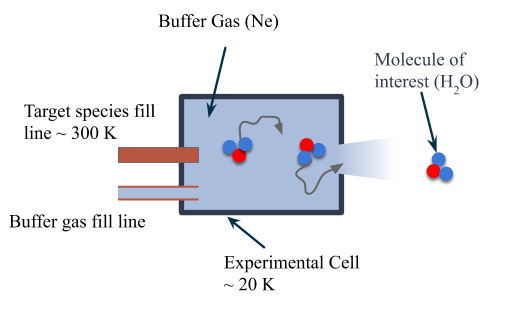
\includegraphics[width=0.6\textwidth]{images/CBGB_diagram.png}
	\caption{Schematic of target species entrainment within a buffer gas beam cell. Introduced target species particles are sympathetically cooled by the buffer gas through elastic collisions where they then may find the exit aperture and produce a beam.}
\end{figure}

Many of the properties of interest are a function of the flow regime of the beam, which is determined by the choice of gas, its flow rate, and the dimensions of the cell it is held in. It's convenient to use the Reynolds number at the aperture to characterize the flow regime, which can be written as:
\begin{align}
	Re & \approx \frac{2 d_{aperture}}{\lambda} \nonumber \\
	& \approx \frac{8\sqrt{2} \dot{N} \sigma}{d_{aperture} \bar{v}} \label{eq: reynolds}
\end{align}
Where $d_{aperture}$ is the diameter of the aperture and $\lambda$ is the mean free path of the buffer gas particles.\cite{Hutzler2012} When the Reynolds number is low, $Re<1$, we find that there are on average $>1$ collisions at the aperture, meaning the particles escape with little to no interactions with other particles and is called the effusive regime. At high Reynolds numbers, $Re>100$, in the supersonic regime, there are many collisions and forward velocity boosting as well as internal velocity distribution narrowing occurs. In between, we find the intermediate regime, where we observe the onset of hydrodynamic entrainment of target species with mild forward velocity boosting. In all cases, the gasses inside the cell at thermal equilibrium follow the Maxwell-Boltzmann distribution.
\begin{equation}
	f(v) = \left(\frac{m}{2 \pi k T}\right)^{3/2}4 \pi v^2 e^{-\frac{m v^2}{2 k T}}
	\label{eq: mb_distribution}
\end{equation}
Where the mean velocity is:
\begin{equation}
	\bar{v} = \sqrt{\frac{8 k_B T}{\pi m}}
	\label{eq: mb_mean}
\end{equation}
The goal for our beam is three fold, to produce a slow, dense, and localized beam of our target species that can make it down into the ion trap region. The velocity and density of the target species are both related to the flow regime of the buffer gas, and to reach our goal, it's ideal for us to aim for a beam that operates within the intermediate regime, between effusive and supersonic. Producing a localized beam ensures that we are introducing the minimal unwanted gas load into the ion trap chamber, and that we may quickly and reliably shutter the beam to start and stop the chemical reactions. In the following sections, we will discuss the design of the apparatus and characterization of the beam density, extraction, forward velocity, and shuttering.